\documentclass[11pt,twocolumn]{article}

\usepackage{graphicx}
\usepackage{amsmath,amssymb}
\usepackage{url}

\usepackage{caption}
\usepackage{subcaption}
\usepackage{parskip}
\setlength {\marginparwidth }{2cm}  % needed to resolve issues
\usepackage{todonotes}
\usepackage[toc,page]{appendix}
\usepackage{hyperref}

%\usepackage[margin=1in,footskip=0.25in]{geometry}

%\newfontfamily{\cyrillicfonttt}{Liberation Mono}

% Margins
%\evensidemargin=0in
%\oddsidemargin=0in
%\textwidth=6.5in

%\setlength{\jot}{8pt}

% Information
\title{Investigating the Viability of Clustering Method in the BdG-formalism}
\author{Axel Tibbling}
\date{ }

\begin{document}

\maketitle

\section{Introduction}\label{sec:introduction}

Blbla what is superconductivity, the importance of the Bardeen–Cooper–Schrieffer (BCS) theory, and leading up to the Bogoliubov-de-Gennes (BdG) formalism (seeing quasiparticles as being in a state representing superconductivity or not). \todo[inline]{Expand on this paragraph}

One can draw associations between the BdG numerical solution method with the Monte Carlo method. Both systems study the total energy of the whole system, and does this for the whole system. Some reserchers saw this as an inefficiency in the Monte Carlo method and realized that only local changes in energy mattered \cite{karmakarDisorderStabilizedBreachedpair2022, kumarTravellingClusterApproximation2006}. \todo[inline]{write this more elaquently}


In this study we employ a similar method for numerical analysis of the BdG Hamiltonian. In section \ref{sec:background} is the BCS model of choice introduced and relevant theory is discussed. Continuing to section \ref{sec:methods} is the normal numerical method for BdG given as well as the proposed cluster method. Results are the given in section \ref{sec:results} and discussed in section \ref{sec:discussion}.  


\section{Background and choice of model}\label{sec:background}

The BdG formalism has its origin in BCS theory, which will act as the starting point. This theory was the first theory to describe superconductivity at a microscopic level, and has been widely accepted in the scientific community as a fundamental description of superconductivity \cite{girvinModernCondensedMatter2019, sharmaReviewTheoriesSuperconductivity2015}. In its essence does it describe an attractive interaction between electrons dominating over the Coloumb force which one would naturally assume to repel electron pairs. 

Interacting electrons form a bounded state which is very stable and does not dissipate energy into the surrounding system. This is a notable observation, as it is one of the key characteristics of superconductors; that electrons does not dissipate their energy, which macroscopicly is seen as resistance.

\subsection{Model of choice}

The system chosen for study is a 1D spin-chain, where the BCS interaction is on-site, and the hopping matrix element is merely neraest neighbor. Chemical potential has also been included. The Hamiltonian for this system is chosen to be 

\begin{align}\label{eq:model}
	H = &-t \sum_{\langle i j\rangle, \sigma}\left(c_{i \sigma}^{\dagger} c_{j \sigma} + c_{j \sigma}^{\dagger} c_{i \sigma}\right) \nonumber \\ 
	    &- V \sum_j n_{j \uparrow} n_{j \downarrow} -\mu \sum_j\left(n_{j \uparrow}+n_{j \downarrow}\right) 
\end{align}

The number operator here is defined as

\begin{equation}
	n_{j, \sigma} = c_{j, \sigma}^\dagger c_{j, \sigma}
\end{equation}

where the first term is the hopping term, the second is the BCS effective, on-site interaction term and the last term is the chemical potential. The latter can be given as a random sequence of numbers to represent impurities in the superconductor. \todo[inline]{will I study impurities?} The $j$ here denote the site at which the operators acts upon and $\sigma$ is the spin of the associated electron (either up or down). The model is a simplifaction of the model used in \cite{zhangChiralPwaveSuperconducting2019} (electron interaction is made on-site). 

\subsection{The Bogoliubov de Gennes formalism}
The Hamiltonian \eqref{eq:model} is given in the basis of normal electrons: $j$ denotes the site of creation/annihilation of said electron. From this only, it is difficult to deduce excitations that correspond to a superconducting state. It would be suitable to transform the basis into a two dimensional one, where one vector corresponds to a \textit{normal} state, and the other corresponds to the excited state, or a \textit{superconducting} state.

This is exactly what Bogoljubov and Valatin realized in 1958 independently in response to the then newly proposed BCS theory \cite{bogoljubovNewMethodTheory1958, valatinCommentsTheorySuperconductivity1958}. What is now considered as the Bogoljubov-Valatin transformation is a transformation of the canonical (anti)commutation relation algebra to one that reflects the state of superconductivity. 


\section{Methods}\label{sec:methods}
\subsection{Normal numerical BdG method}
\subsection{Cluster BdG method}

\section{Results}\label{sec:results}

\begin{figure}[ht!]
	\centering
	\begin{subfigure}{0.5\textwidth}
	\begin{center}
		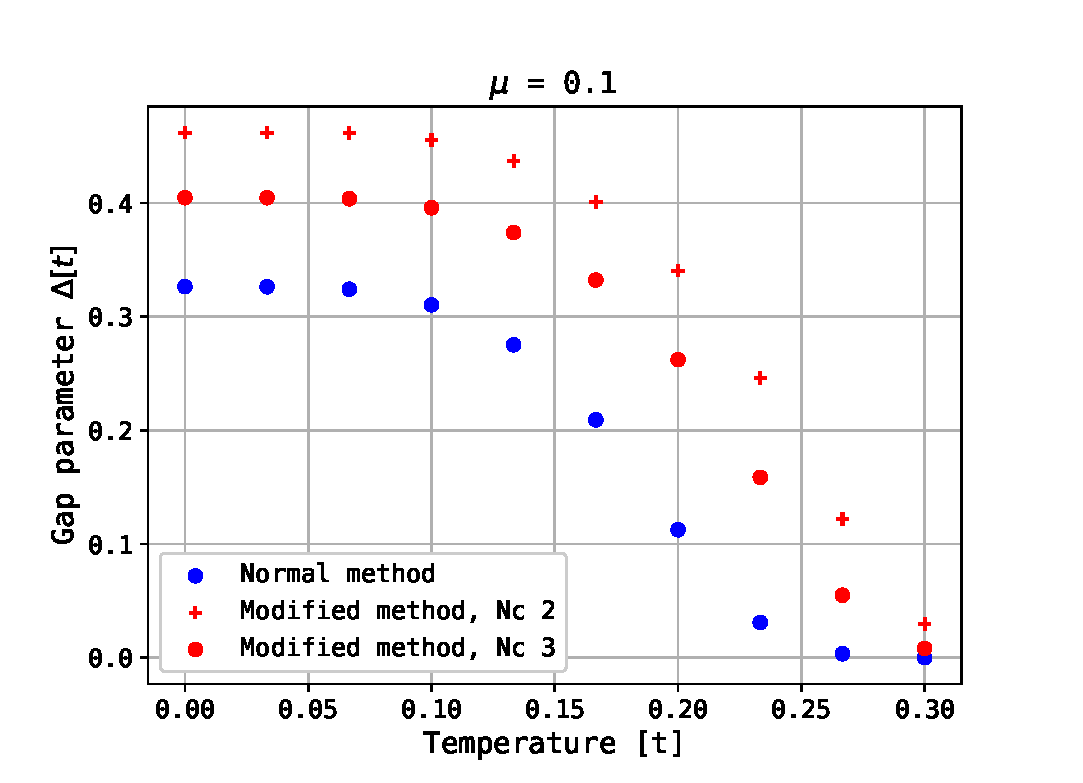
\includegraphics[width=\textwidth]{figures/deltacomp_N30_mu0.1.eps}
	\end{center}
	\end{subfigure}
	\begin{subfigure}{0.5\textwidth}
	\begin{center}
		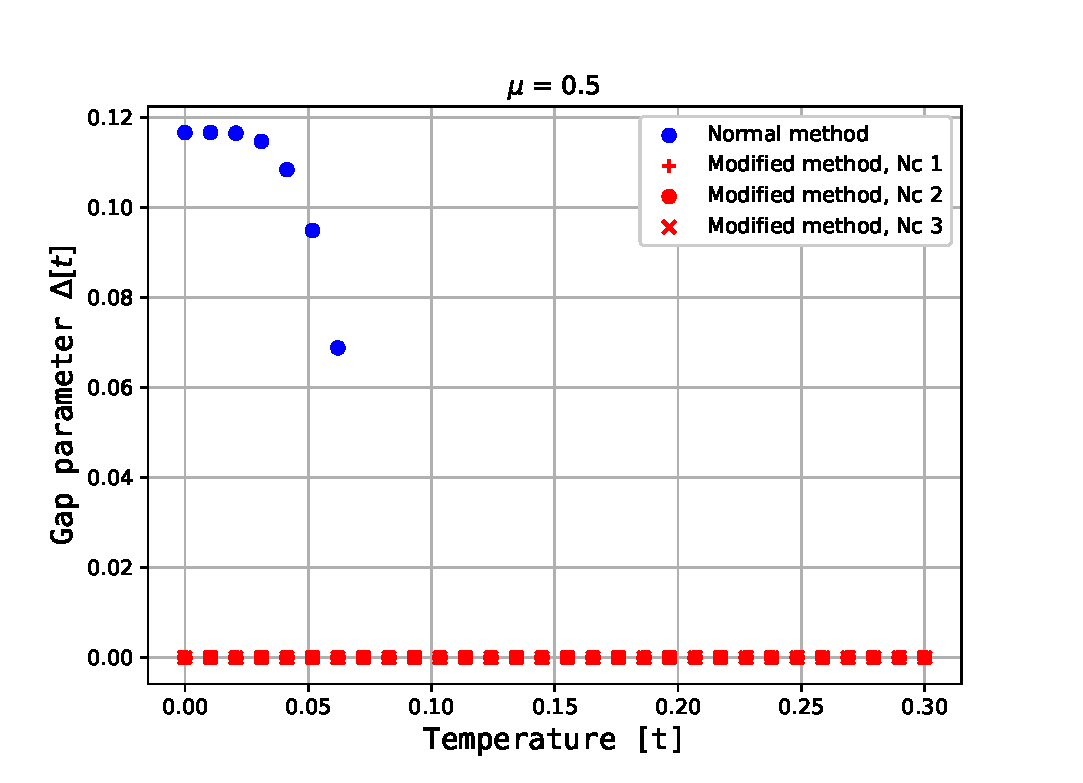
\includegraphics[width=\textwidth]{figures/deltacomp_N30_mu0.5.eps}
	\end{center}
	\end{subfigure}
	\caption{The graph}
	\label{fig:thegraph}
\end{figure}

\section{Discussion}\label{sec:discussion}


\onecolumn
% ref
\bibliographystyle{plain} % We choose the "plain" reference style
\bibliography{refs} % Entries are in the refs.bib file

\end{document}

pdflatex: --aux-directory=build
bibtex: build/% -use-directory=build

